\documentclass[12pt]{book}

\usepackage[a4paper, portrait, margin=0.75in]{geometry}
\usepackage{graphicx} % Required for inserting images
\usepackage[page,toc,titletoc,title]{appendix}
\usepackage{mathptmx}
\usepackage{pdflscape}
\usepackage{pdfpages}
\usepackage{enumitem}
\usepackage{hyperref}
\usepackage{cleveref}

\title{Integrating streamed sensor data into a distributed model of a complex system \\
\large{A report submitted in partial fulfilment of the requirements for the degree of \\
\textbf{Bachelor of Engineering (Hons) in Software Engineering} \\
at \\
\textbf{the University of Waikato}
}}

\author{Bert Downs  \\ 
Supervised by Tim Walmsley, Mark Apperley }

\date{October 2024}

\begin{document}

\maketitle

\newpage

\chapter*{Abstract}

Modern factories are equipped with a variety of sensors that monitor the state of the factory and products. To fully utilise this sensor data, the field of Digital Twinning is emerging, which combines live factory data, historical state, and a model of the factory to predict future states. The process of creating a digital twin lacks standardization. This project develops a standardised framework for creating digital twins of chemical plants, using the Ahuora Digital Twin Platform and industry standard data processing tools.  

% TODO: Something about results and evaluation stuff.

\newpage
\tableofcontents



\newpage




\chapter{Introduction}



\bibliographystyle{unsrt} % We choose the "plain" reference style
\bibliography{refs} % Entries are in the refs.bib file

\begin{appendices}



% \chapter{Project Proposal} \label{sec:proposal}
% The project proposal is included as an appendix on the following page.


% 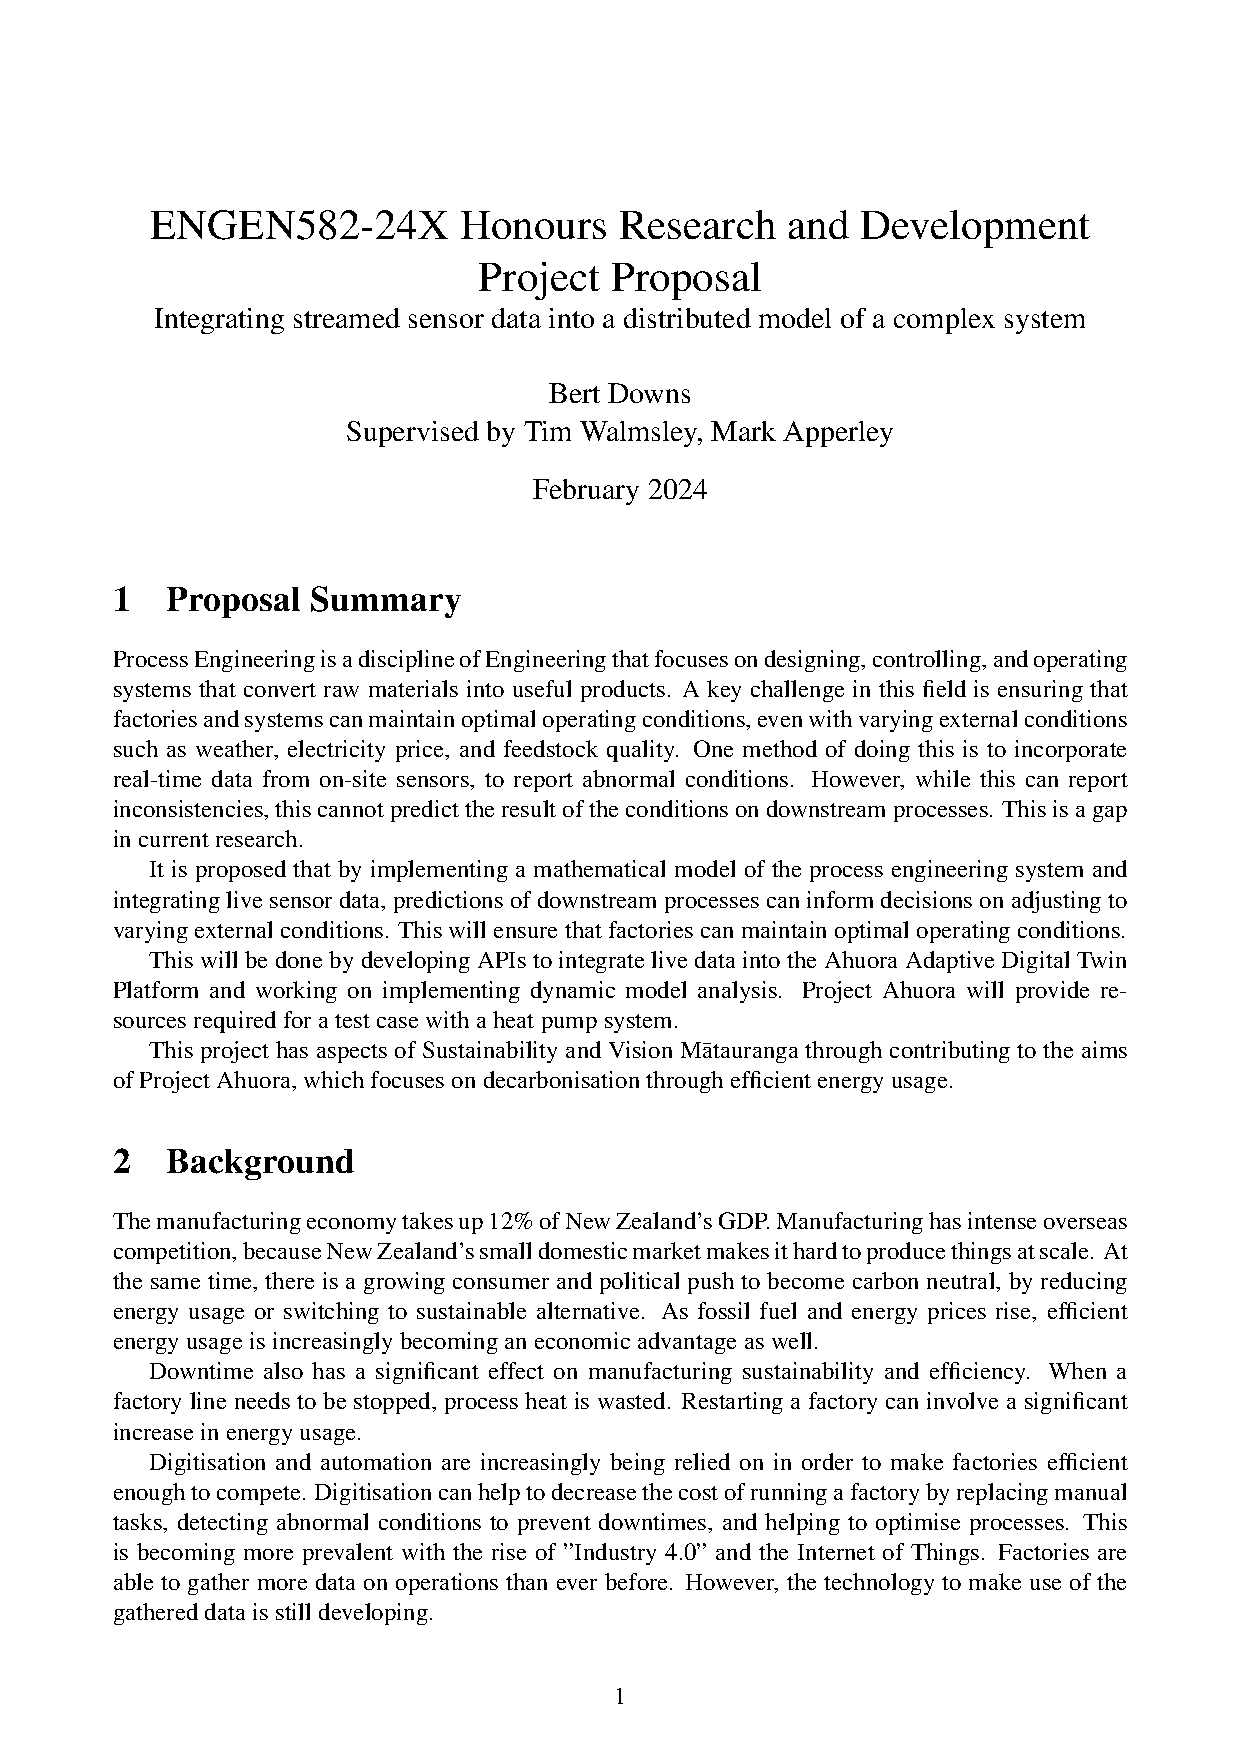
\includepdf[pages=1-4]{proposal.pdf}

% \begin{landscape}
%     \includepdf[pages=5,angle=90]{proposal.pdf}
% \end{landscape}

% \chapter{Literature Review} \label{sec:litreview}
% The literature review is included as an appendix on the following page.

% 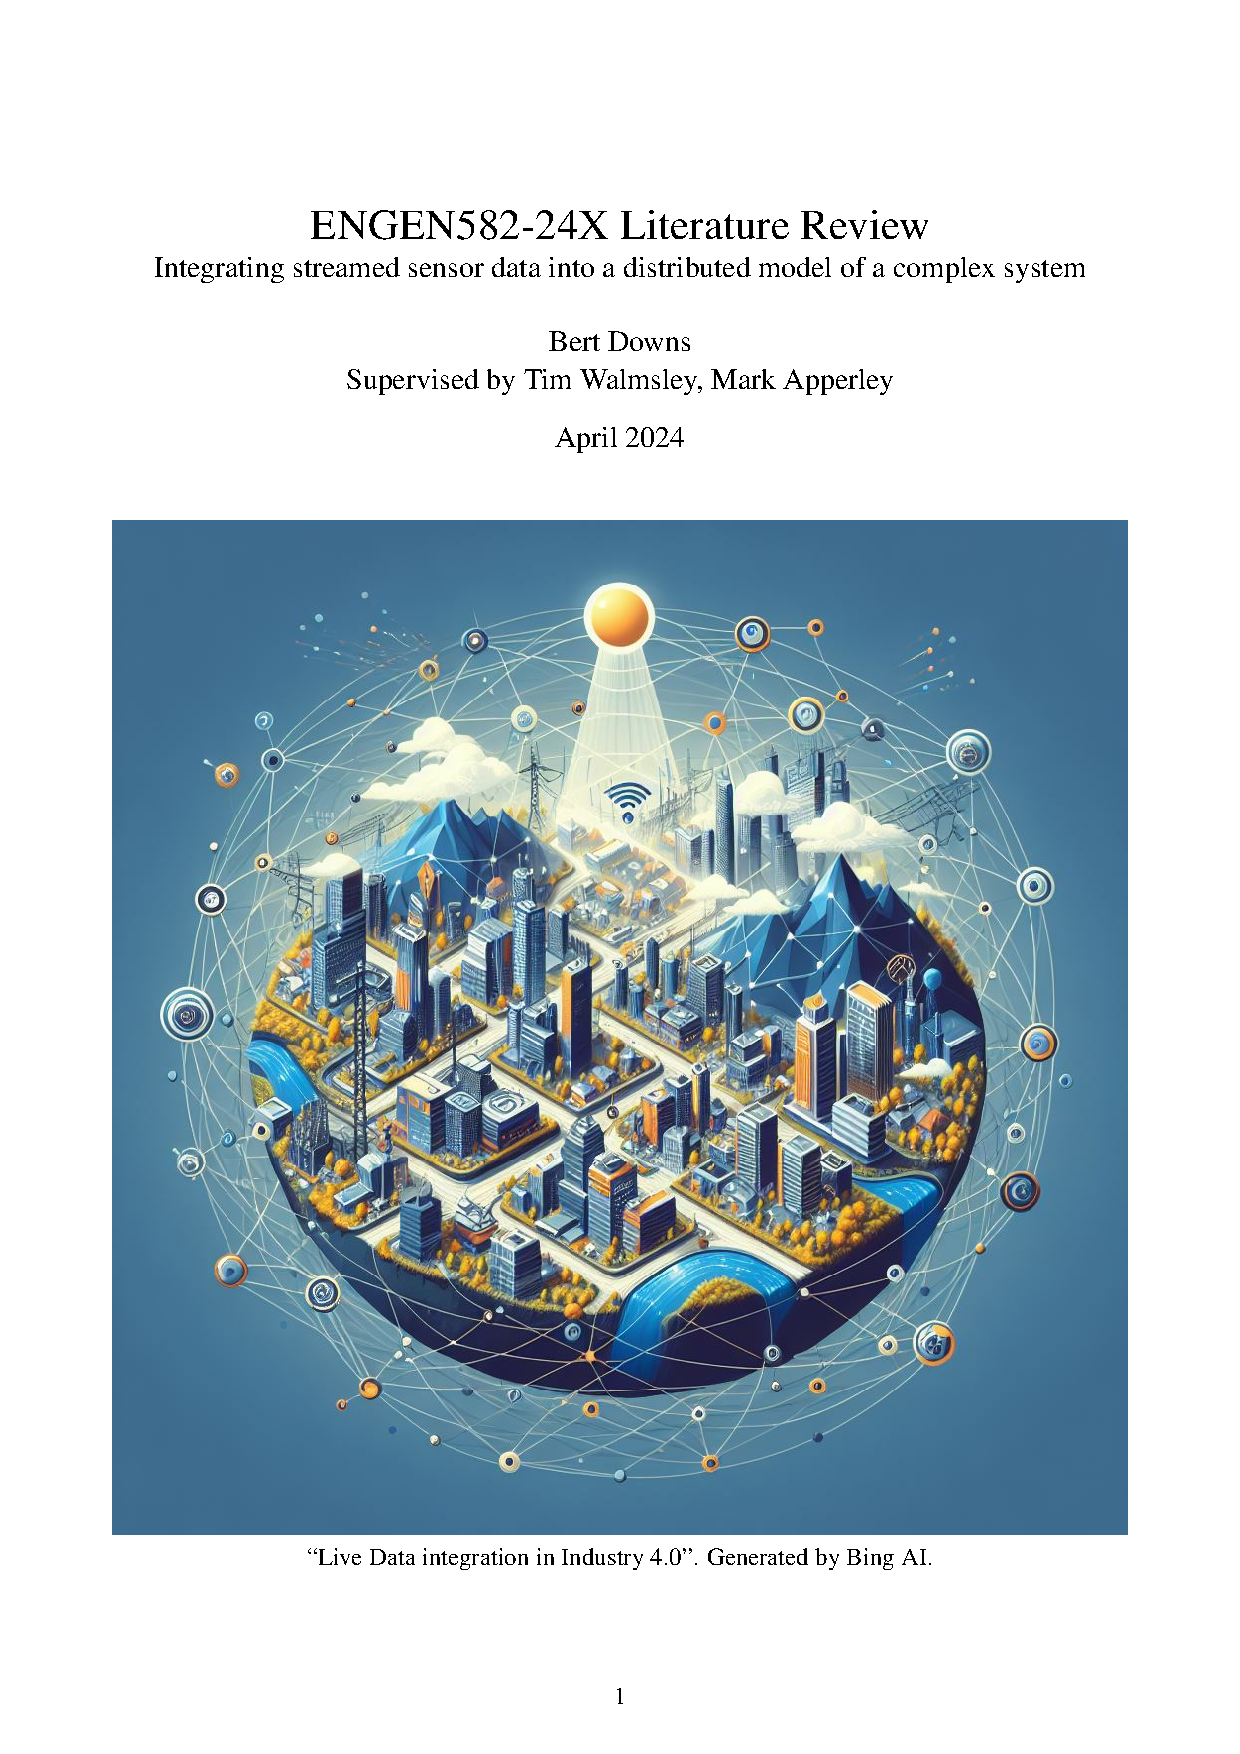
\includepdf[pages=-]{literature_review.pdf}

\end{appendices}
\end{document}